\begin{appendix}
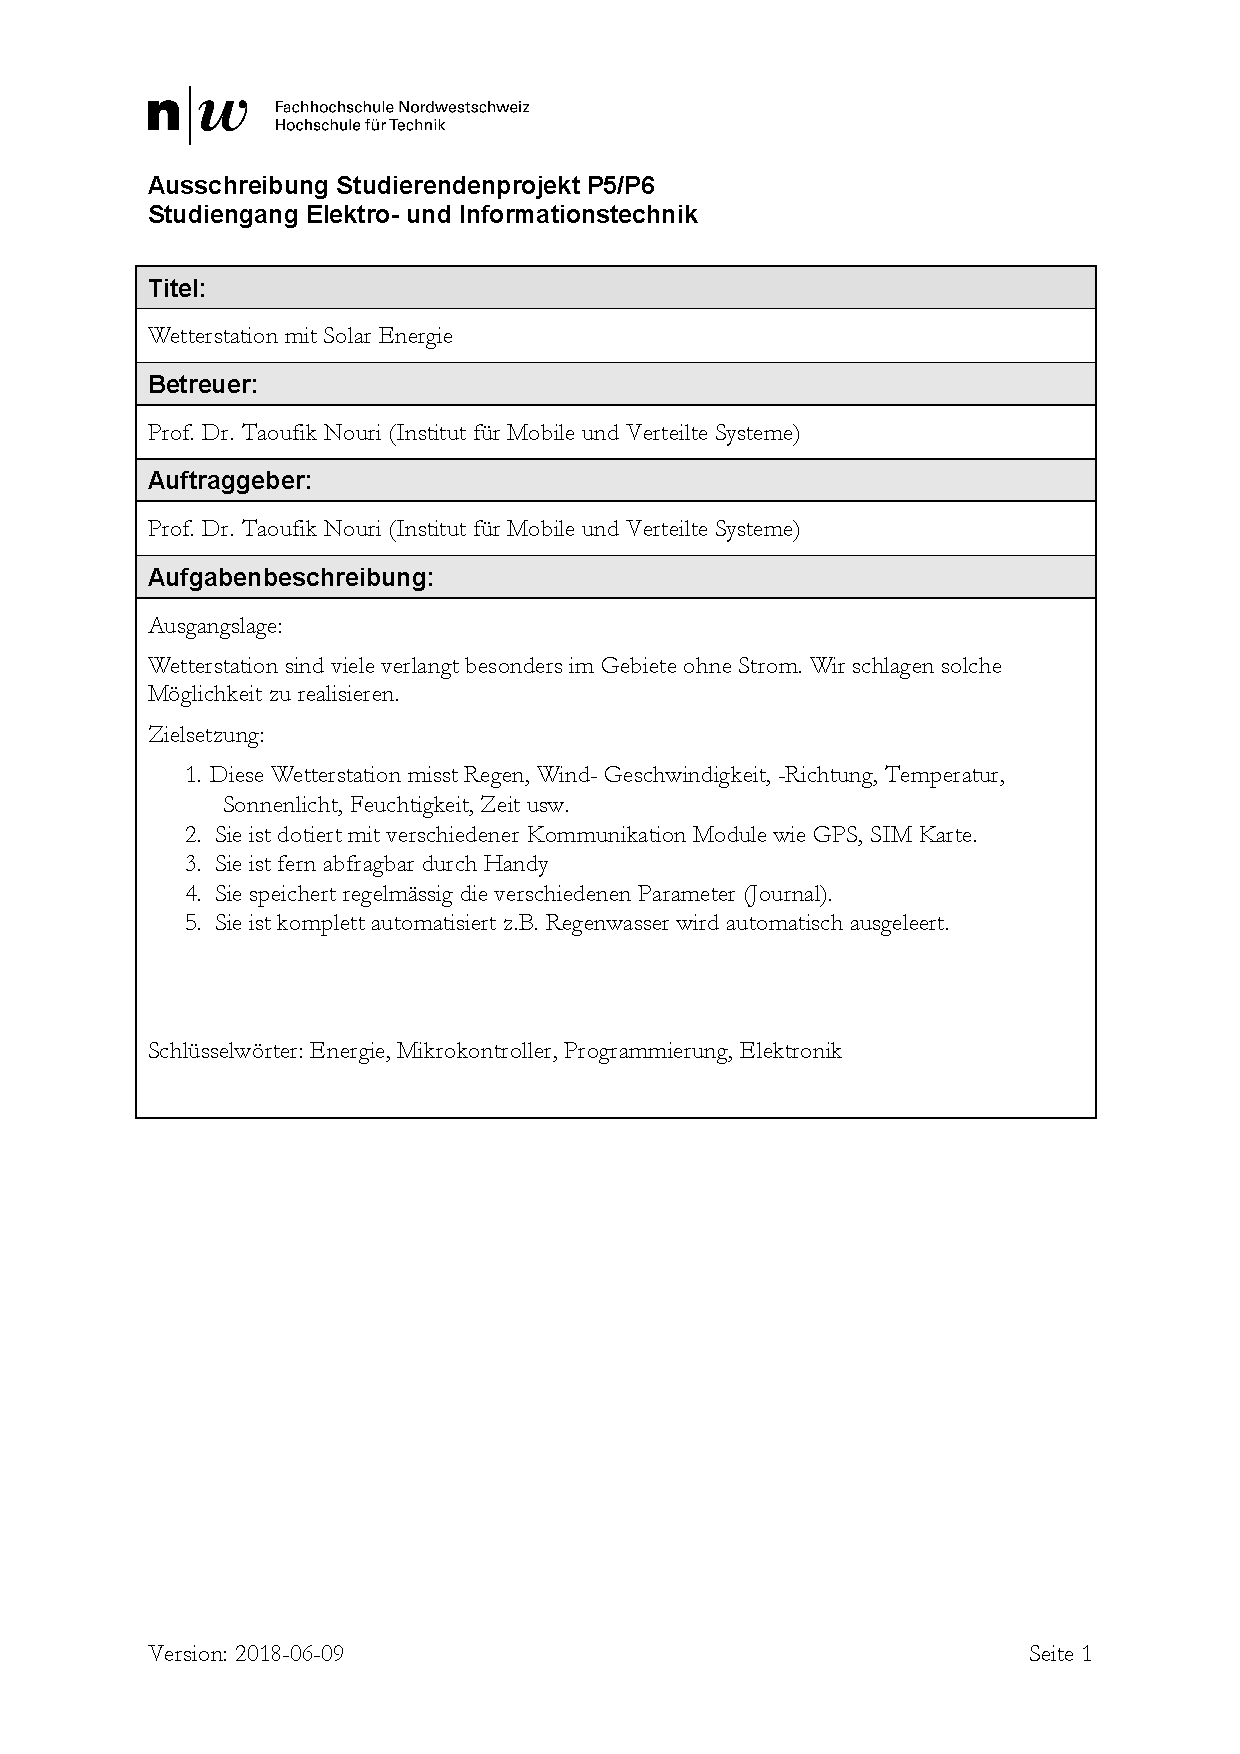
\includepdf[pages={1},nup=1x1,landscape=false,scale=0.85,offset=0 -40,pagecommand={\section{Lastenheft}\label{tab:zeitplan}\thispagestyle{myheadings}}]{appendix/Auftragsbeschreibung.pdf} 
\newpage

\section{ATmega2560-Arduino Pin Mapping}
\label{sec:pinMapping}
\begin{table}[h]
  \centering
  \caption{ATmega2560-Arduino Pin Mapping Tabelle \cite{ArduinoPinMapping2018}}
    \begin{tabular}{|c|p{15.855em}|p{11.43em}|}
    \hline
    \multicolumn{1}{|p{7.07em}|}{\textbf{Pin Number}} & \textbf{Pin Name} & \textbf{Mapped Pin Name} \\
    \hline
    1     & PG5 ( OC0B ) & Digital pin 4 (PWM) \\
    \hline
    2     & PE0 ( RXD0/PCINT8 ) & Digital pin 0 (RX0) \\
    \hline
    3     & PE1 ( TXD0 ) & Digital pin 1 (TX0) \\
    \hline
    4     & PE2 ( XCK0/AIN0 ) & \multicolumn{1}{l|}{} \\
    \hline
    5     & PE3 ( OC3A/AIN1 ) & Digital pin 5 (PWM) \\
    \hline
    6     & PE4 ( OC3B/INT4 ) & Digital pin 2 (PWM) \\
    \hline
    7     & PE5 ( OC3C/INT5 ) & Digital pin 3 (PWM) \\
    \hline
    8     & PE6 ( T3/INT6 ) & \multicolumn{1}{l|}{} \\
    \hline
    9     & PE7 ( CLKO/ICP3/INT7 ) & \multicolumn{1}{l|}{} \\
    \hline
    10    & VCC   & VCC \\
    \hline
    11    & GND   & GND \\
    \hline
    12    & PH0 ( RXD2 ) & Digital pin 17 (RX2) \\
    \hline
    13    & PH1 ( TXD2 ) & Digital pin 16 (TX2) \\
    \hline
    14    & PH2 ( XCK2 ) & \multicolumn{1}{l|}{} \\
    \hline
    15    & PH3 ( OC4A ) & Digital pin 6 (PWM) \\
    \hline
    16    & PH4 ( OC4B ) & Digital pin 7 (PWM) \\
    \hline
    17    & PH5 ( OC4C ) & Digital pin 8 (PWM) \\
    \hline
    18    & PH6 ( OC2B ) & Digital pin 9 (PWM) \\
    \hline
    19    & PB0 ( SS/PCINT0 ) & Digital pin 53 (SS) \\
    \hline
    20    & PB1 ( SCK/PCINT1 ) & Digital pin 52 (SCK) \\
    \hline
    21    & PB2 ( MOSI/PCINT2 ) & Digital pin 51 (MOSI) \\
    \hline
    22    & PB3 ( MISO/PCINT3 ) & Digital pin 50 (MISO) \\
    \hline
    23    & PB4 ( OC2A/PCINT4 ) & Digital pin 10 (PWM) \\
    \hline
    24    & PB5 ( OC1A/PCINT5 ) & Digital pin 11 (PWM) \\
    \hline
    25    & PB6 ( OC1B/PCINT6 ) & Digital pin 12 (PWM) \\
    \hline
    26    & PB7 ( OC0A/OC1C/PCINT7 ) & Digital pin 13 (PWM) \\
    \hline
    27    & PH7 ( T4 ) & \multicolumn{1}{l|}{} \\
    \hline
    28    & PG3 ( TOSC2 ) & \multicolumn{1}{l|}{} \\
    \hline
    29    & PG4 ( TOSC1 ) & \multicolumn{1}{l|}{} \\
    \hline
    30    & RESET & RESET \\
    \hline
    31    & VCC   & VCC \\
    \hline
    32    & GND   & GND \\
    \hline
    33    & XTAL2 & XTAL2 \\
    \hline
    34    & XTAL1 & XTAL1 \\
    \hline
    35    & PL0 ( ICP4 ) & Digital pin 49 \\
    \hline
    \end{tabular}%
  \label{tab:ATmega2560-Arduino Pin Mapping Tabelle}%
\end{table}%
\newpage
% Table generated by Excel2LaTeX from sheet 'Tabelle1'
\begin{table}[h]
  \centering
    \begin{tabular}{|c|p{15.855em}|p{11.43em}|}
    \hline
    \multicolumn{1}{|p{7.07em}|}{\textbf{Pin Number}} & \textbf{Pin Name} & \textbf{Mapped Pin Name} \\
    \hline
    36    & PL1 ( ICP5 ) & Digital pin 48 \\
    \hline
    37    & PL2 ( T5 ) & Digital pin 47 \\
    \hline
    38    & PL3 ( OC5A ) & Digital pin 46 (PWM) \\
    \hline
    39    & PL4 ( OC5B ) & Digital pin 45 (PWM) \\
    \hline
    40    & PL5 ( OC5C ) & Digital pin 44 (PWM) \\
    \hline
    41    & PL6   & Digital pin 43 \\
    \hline
    42    & PL7   & Digital pin 42 \\
    \hline
    43    & PD0 ( SCL/INT0 ) & Digital pin 21 (SCL) \\
    \hline
    44    & PD1 ( SDA/INT1 ) & Digital pin 20 (SDA) \\
    \hline
    45    & PD2 ( RXDI/INT2 ) & Digital pin 19 (RX1) \\
    \hline
    46    & PD3 ( TXD1/INT3 ) & Digital pin 18 (TX1) \\
    \hline
    47    & PD4 ( ICP1 ) & \multicolumn{1}{l|}{} \\
    \hline
    48    & PD5 ( XCK1 ) & \multicolumn{1}{l|}{} \\
    \hline
    49    & PD6 ( T1 ) & \multicolumn{1}{l|}{} \\
    \hline
    50    & PD7 ( T0 ) & Digital pin 38 \\
    \hline
    51    & PG0 ( WR ) & Digital pin 41 \\
    \hline
    52    & PG1 ( RD ) & Digital pin 40 \\
    \hline
    53    & PC0 ( A8 ) & Digital pin 37 \\
    \hline
    54    & PC1 ( A9 ) & Digital pin 36 \\
    \hline
    55    & PC2 ( A10 ) & Digital pin 35 \\
    \hline
    56    & PC3 ( A11 ) & Digital pin 34 \\
    \hline
    57    & PC4 ( A12 ) & Digital pin 33 \\
    \hline
    58    & PC5 ( A13 ) & Digital pin 32 \\
    \hline
    59    & PC6 ( A14 ) & Digital pin 31 \\
    \hline
    60    & PC7 ( A15 ) & Digital pin 30 \\
    \hline
    61    & VCC   & VCC \\
    \hline
    62    & GND   & GND \\
    \hline
    63    & PJ0 ( RXD3/PCINT9 ) & Digital pin 15 (RX3) \\
    \hline
    64    & PJ1 ( TXD3/PCINT10 ) & Digital pin 14 (TX3) \\
    \hline
    65    & PJ2 ( XCK3/PCINT11 ) & \multicolumn{1}{l|}{} \\
    \hline
    66    & PJ3 ( PCINT12 ) & \multicolumn{1}{l|}{} \\
    \hline
    67    & PJ4 ( PCINT13 ) & \multicolumn{1}{l|}{} \\
    \hline
    68    & PJ5 ( PCINT14 ) & \multicolumn{1}{l|}{} \\
    \hline    
    69    & PJ6 ( PCINT 15 ) & \multicolumn{1}{l|}{} \\
    \hline
    70    & PG2 ( ALE ) & Digital pin 39 \\
    \hline
    71    & PA7 ( AD7 ) & Digital pin 29 \\
    \hline
    72    & PA6 ( AD6 ) & Digital pin 28 \\
    \hline
    73    & PA5 ( AD5 ) & Digital pin 27 \\
    \hline
    74    & PA4 ( AD4 ) & Digital pin 26 \\
    \hline
    75    & PA3 ( AD3 ) & Digital pin 25 \\
    \hline
    76    & PA2 ( AD2 ) & Digital pin 24 \\
    \hline
    77    & PA1 ( AD1 ) & Digital pin 23 \\
    \hline
    78    & PA0 ( AD0 ) & Digital pin 22 \\
    \hline
    79    & PJ7   & \multicolumn{1}{l|}{} \\
    \hline
    80    & VCC   & VCC \\
    \hline
    \end{tabular}%
\end{table}%
% Table generated by Excel2LaTeX from sheet 'Tabelle1'
\begin{table}[h]
  \centering
    \begin{tabular}{|c|p{15.855em}|p{11.43em}|}
    \hline
    \multicolumn{1}{|p{7.07em}|}{\textbf{Pin Number}} & \textbf{Pin Name} & \textbf{Mapped Pin Name} \\
    \hline
    81    & GND   & GND \\
    \hline
    82    & PK7 ( ADC15/PCINT23 ) & Analog pin 15 \\
    \hline
    83    & PK6 ( ADC14/PCINT22 ) & Analog pin 14 \\
    \hline
    84    & PK5 ( ADC13/PCINT21 ) & Analog pin 13 \\
    \hline
    85    & PK4 ( ADC12/PCINT20 ) & Analog pin 12 \\
    \hline
    86    & PK3 ( ADC11/PCINT19 ) & Analog pin 11 \\
    \hline
    87    & PK2 ( ADC10/PCINT18 ) & Analog pin 10 \\
    \hline
    88    & PK1 ( ADC9/PCINT17 ) & Analog pin 9 \\
    \hline
    89    & PK0 ( ADC8/PCINT16 ) & Analog pin 8 \\
    \hline
    90    & PF7 ( ADC7 ) & Analog pin 7 \\
    \hline
    91    & PF6 ( ADC6 ) & Analog pin 6 \\
    \hline
    92    & PF5 ( ADC5/TMS ) & Analog pin 5 \\
    \hline
    93    & PF4 ( ADC4/TMK ) & Analog pin 4 \\
    \hline
    94    & PF3 ( ADC3 ) & Analog pin 3 \\
    \hline
    95    & PF2 ( ADC2 ) & Analog pin 2 \\
    \hline
    96    & PF1 ( ADC1 ) & Analog pin 1 \\
    \hline
    97    & PF0 ( ADC0 ) & Analog pin 0 \\
    \hline
    98    & AREF  & Analog Reference \\
    \hline
    99    & GND   & GND \\
    \hline
    100   & AVCC  & VCC \\
    \hline
    \end{tabular}%
\end{table}%

\begin{figure}[h]
\centering
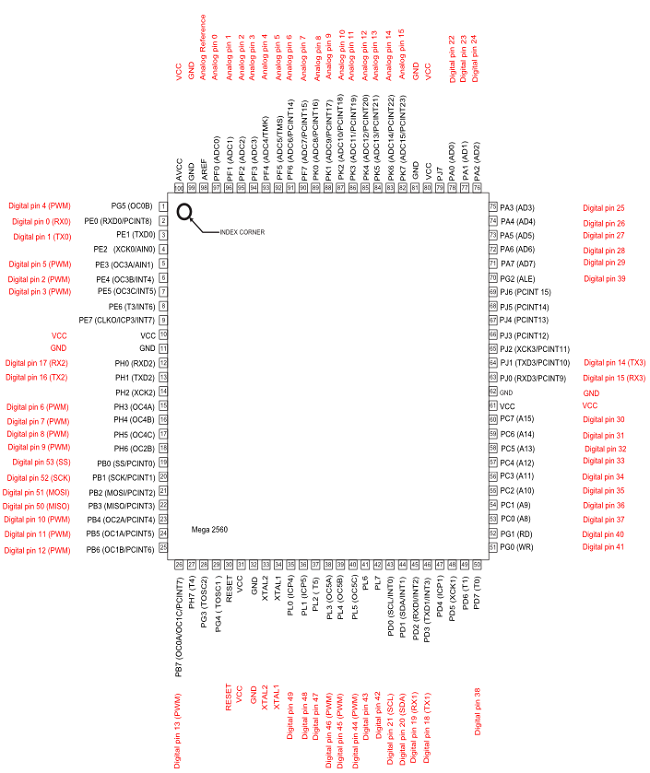
\includegraphics[width=\textwidth]{graphics/MCU/atmega2560_pins.png}
\caption{ATmega2560 Pin Layout}
\label{fig:ATmega2560PinLayout}
\end{figure}


\end{appendix}